\normaltrue
\correctionfalse

%\UPSTIidClasse{11} % 11 sup, 12 spé
%\newcommand{\UPSTIidClasse}{12}

\exer{Mouvement RT  $\star$ \label{CIN:01:B2:12:06}}
\setcounter{question}{0}\marginnote{\xpComp{CIN}{01}}%\UPSTIcompetence{B2-12}
\index{Compétence B2-12}\index{Compétence CIN-01}
\index{Mécanisme à 1 translation et 1 rotation}
\ifcorrection
\else
\marginnote{\textbf{Pas de corrigé pour cet exercice.}}
\fi

\ifprof
\else
Soit le mécanisme suivant. On a $\vect{AB}=\lambda(t)\vect{i_0}$ et $\vect{BC}=R\vect{i2}$.
\begin{marginfigure}
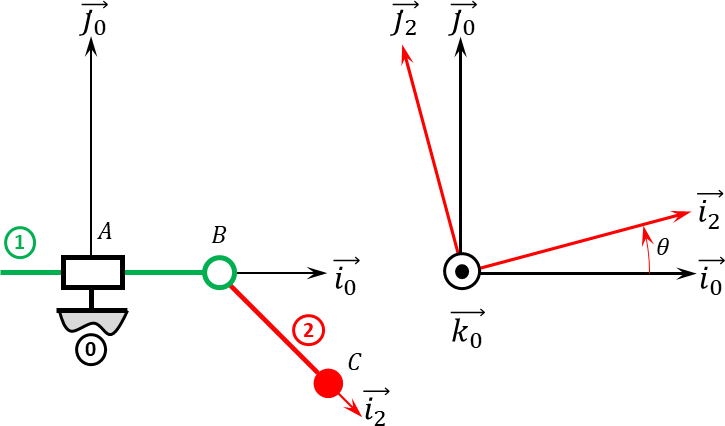
\includegraphics[width=\linewidth]{06_TR_01}
\end{marginfigure}
\fi

\question{Tracer le graphe des liaisons.}
\ifprof
\else
\fi

\question{Retracer le schéma cinématique pour $\theta=\dfrac{\pi}{4}\,\text{rad}$ et $\lambda(t)=\SI{20}{mm}$.}
\ifprof
\else
\fi

\question{Retracer le schéma cinématique pour $\theta=\dfrac{-\pi}{4}\,\text{rad}$ et $\lambda(t)=-\SI{20}{mm}$.}
\ifprof
\else
\fi



\ifprof
\else

\marginnote{Corrigé  voir \ref{CIN:01:B2:12:06}.}

\fi